% 2009 年广东卷（理科）第 15 题：圆 O 上三点 A、B、C，AB=4，∠ACB=45°。
% 来源 PDF：.work/ocr-local/sources/2009广东理.pdf
% SHA-256：5256b35235a042e254d36c111af3eda0f5dd8f552664021d0bace5c05582ad04
% 原页：第 1 页（A3 四栏）第 3 栏，印刷页 519。
% 绘制依据：AB 为竖直弦（B 在右上、A 在右下），C 在下方，连 CA、CB；
%   圆周角 ∠ACB=45° 对应 AB 所对圆心角 90°。
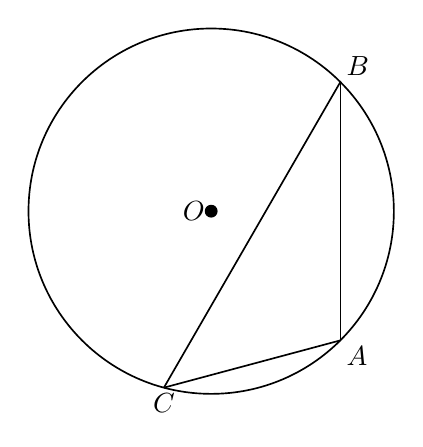
\begin{tikzpicture}[scale=1.45, semithick, every node/.style={inner sep=2pt}]
  \draw (0,0) circle (1.6);
  \coordinate (O) at (0,0);
  \coordinate (B) at (45:1.6);
  \coordinate (A) at (-45:1.6);
  \coordinate (C) at (255:1.6);

  \draw (A) -- (B);
  \draw (C) -- (B);
  \draw (C) -- (A);

  \fill (O) circle (1.6pt);
  \node[left] at (0,0) {$O$};
  \node[above right] at (B) {$B$};
  \node[below right] at (A) {$A$};
  \node[below] at (C) {$C$};
\end{tikzpicture}
